\chapter[Measuring completeness as metadata quality metric in Europeana]{Measuring completeness as metadata quality metric in Europeana\footnote{This chapter has been first published as extended abstract in Digital Humanities 2017 Conference
Abstracts (\url{https://dh2017.adho.org/abstracts/DH2017-abstracts.pdf}) then as a full paper: \cite{kiraly2018}}}
\chapterauthor{Péter Király and Marco Büchler\footnote{Péter Király created the experiments, the underlying software, and contributed to the text. Marco Büchler contributed to the text.}}

\emph{Abstract}: Europeana, the European digital platform for cultural heritage, has a heterogeneous collection of metadata records ingested from more than 3200 data providers. The original nature and context of these records was different. In order to create effective services upon this data it is important to know the strengths and weaknesses, or in other words, the quality of these data. This chapter proposes a method and an open source implementation to reveal quality issues by measuring some structural features of these data, such as completeness, multilinguality, uniqueness, and record patterns.

%\begin{IEEEkeywords}
Big data applications, Data analysis, Data collection, Quality of service, Quality management, Metadata, Data integration
%\end{IEEEkeywords}

\section{Introduction}

\begin{displayquote}
"In the last 24 hours, I wasted a lot of time because I made assumptions about some (meta)data that were just not correct. I spend a long time debugging, but the code was fine, it just couldn’t find what’s not there. Wrong assumptions are some of the most difficult bugs to catch." -- Felix Rau, German linguist on the consequence of metadata issues\footnote{18 Oct 2018, \url{https://twitter.com/fxru/status/1052838758066868224}}
\end{displayquote}
Big data applications, Data analysis, Data collection, Quality of service, Quality management 
\bigskip

The functionalities of an aggregated metadata collection are dependent on the quality of metadata records. Some examples from Europeana, the European digital platform for cultural heritage\footnote{http://europana.eu}, illustrate the importance of metadata:

(a) Several thousand records have the title 'Photo' or its synonyms across language variations without further description; how can a user find  objects which depict a particular building in these photos if either no or only imprecise textual descriptions are available?

(b) Several data providers are listed in Europeana's 'Institution' facet under multiple name variants (e.g. 'Cinecittà Luce S.p.A.' (372,412 records), 'Cinecittà Luce' (2,405 records), 'LUCE' (105 records)  refer to the same organization). Do we expect a user to select all variant forms when s/he wants to search for objects belonging to a particular organization?

(c) Without formalized and unified values in the 'year' facet, we are not able to use the functionality of interactive date range selectors. How can we interpret values such as '13436', or '97500000' when we expect a year?

(d) Some records have only technical identifiers, without any descriptive fields (title, creator, description, subjects, etc.). These records are not human readable and do not support any of the core functionalities of Europeana.

(e) In a multilingual environment the user would expect that s/he would get the same result-set when searching for a well-known entity, such as Leonardo's masterpiece 'Mona Lisa' (or 'La Gioconda', 'La Joconde'), however, the different language variations return different result-sets and are not resolved into a common entity.

The question is thus how to decide which records should be improved, and which are good enough? 'Fitness for purpose' is a well-known slogan of quality assurance, referring to the concept that quality should be defined according to some business purpose. When dealing with metadata quality it is relevant to clarify why metadata are important. In Europeana's case it is relatively straightforward in that it provides access points to digitized objects. If the features of a record make it impossible to find an object then its intended purpose is not met as the user cannot use an object they cannot access. One could then reasonably argue that the quality of such a record is insufficient. The manual evaluation of each record, however, is not affordable for even a middle-size collection.

This chapter proposes a generalized methodology and a scalable software package which can be used in Europeana and elsewhere in the cultural heritage domain for either big or small data collections.

\section{Background and foundations}

Europeana collects and presents cultural heritage metadata records. The database at the time of this writing contains more than 58 million records in the Europeana Data Model (EDM) metadata schema from more than 3200 institutions\footnote{Extracted from Europeana Search API.} i. The organizations can send their data in EDM or in another metadata standard. Due to the variety of original data formats, cataloguing rules, languages and vocabularies, there are large differences in the quality of individual records, which heavily affects Europeana's service functionalities.

In 2015, a Europeana task force investigated the problem of metadata quality, and published a report (see \cite{dangerfield2015}), however -- as stated -- `there was not enough scope … to investigate … metrics for metadata quality ….' In 2016, a wider Data Quality Committee\footnote{https://pro.europeana.eu/project/data-quality-committee} (DQC) was founded and several experts on this committee from different domains (such as metadata theory, cataloguing, academic research, software development) came together to analyse and revise the metadata schema, discuss data normalization, run functional requirements analysis and define 'enabling' elements (answering questions such as 'What are the core functionalities of Europeana?' and 'Which metadata elements support them?'). DQC also built a ‘problem catalogue’, which is a collection of frequently occurring metadata anti-patterns (such as duplicate values, title field repeated as description, values for machine consumption in fields which were intended for human consumption, etc.) \cite{hill-manguinhas2016}. The questions of multilinguality were given special emphasis.

This current research is being conducted in collaboration with the DQC with the purpose of finding methods, defining metrics and building an open source tool called 'Metadata Quality Assurance Framework'\footnote{http://144.76.218.178/europeana-qa/, source code and background information: http://pkiraly.github.io} to measure metadata quality. The proposed method is intended to be a generic tool for measuring metadata quality. It is adaptable to different metadata schemas (planned schemas include – but are not limited to – MARC\footnote{MAchine Readable Cataloging, https://www.loc.gov/marc/. A MARC assessment tool based on this framework is also created. It is available at https://github.com/pkiraly/metadata-qa-marc. Note that MARC is a much more complex standard than EDM, and the presence of a strict rule-set makes finding individual problems more important than in the case of Europeana records, so there are more emphasis on the "accuracy" and "conformance to expectation" metrics.} and Encoded Archival Description\footnote{http://www.loc.gov/ead/}). The software is scalable to Big Data, as it is built to work together with the distributed file system of Apache Hadoop\footnote{http://hadoop.apache.org/}, the general, large-scale data processing engine Apache Spark\footnote{http://spark.apache.org/}, and the Apache Cassandra\footnote{http://cassandra.apache.org/} database. One of the most important features of this approach is the capability to produce reports understandable to data curators, who are not familiar with the language used by software developers, data scientists or statisticians. The reports are generated for those who are then able to turn them into actionable plans. The framework is modular: there is a schema-independent core library with schema specific extensions. It is designed for usage in continuous integration for metadata quality assessment.\footnote{See http://pkiraly.github.io/2016/07/02/making-general/ and \cite{kiraly2017}}

The research discussed here questions how the quality of cultural heritage metadata can be best measured. It is generally assumed that quality itself is too complex for a single concept, and that it is impossible to measure every aspect of it both for theoretical reasons (for example current language detection methods do not work well with the short texts typically available in metadata records) and for practical reasons (such as limited resources). A number of structural features of the metadata record, however, are measurable and the outcome provides a good approximation in most cases. One could call it ‘metadata smells’, similar to what is called 'code smells' in software development: 'a surface indication that usually corresponds to a deeper problem in the system'.\footnote{The term was coined by Kent Beck and popularized by Martin Fowler in his Refactoring book, see https://martinfowler.com/bliki/CodeSmell.html} Approximation means in practice that the outcome should call for further scrutiny by metadata experts. It also implies that there is a fair chance that the tool cannot detect variances due to those errors that are not bound to structural features.

The primary purpose of the project is to shed light on improvable metadata records. If we know where the errors are, then we can prioritize what needs to be fixed first and corrections to metadata can be planned in order of the importance of the problem. Since Europeana is an aggregator, corrections should be made at the information source itself, inside the database of the particular data provider. Better data supports more reliable functions, so by fixing weak records Europeana could build stronger services. Finding typical errors might also help improve the underlying metadata schema and its documentation (supposedly some of the errors occurred due to the language used in the schema documentation).  In addition, during the measurement process examples of bad and good practice for certain metadata elements could be found and highlighted. Lastly high scoring metadata records could be used to propagate 'good metadata practices' or assist in the process of prototyping new services.

\section{State of the art}

The computational methods for metadata quality assessment emerged in the last decade in the cultural heritage domain (\cite{bruce-hillmann2004}, \cite{stvilia2007}, \cite{ochoa-duval2009}, \cite{harper2016}). The latest evaluation of the relevant work was conducted by \cite{palavitsinis2014}. The applied metrics in the domain of Linked Data (which has an intersection with the cultural heritage domain) are listed in \cite{zaveri2015}. While some papers defined quality metrics others suggested computational implementations. Nonetheless, they mostly analyzed smaller volumes of records, metadata schemas which are less complex than EDM, and usually applied methods to more homogeneous data sets (notable exceptions are \cite{newman2007} investigating 7 million, and \cite{harper2016} investigating 25 million records). The novelty of this research is that it increases the volume of records, introduces new types of data visualizations and quality reports, and provides an open source implementation that is reusable in other collections.

For a comprehensive bibliography of cultural heritage metadata assessment see the Metadata Assessment Zotero library\footnote{http://zotero.org/groups/metadata\_assessment} which is maintained by the members of the Digital Library Federation’s Metadata Assessment group\footnote{https://dlfmetadataassessment.github.io/} and members of the DQC including the first author of this chapter.

\section{Methodology}

\subsection{The EDM schema}

An EDM record\footnote{For EDM documentation, guidelines and other materials consult https://pro.europeana.eu/page/edm-documentation} consists of several entities. The core of the record is called the \emph{provider proxy}, it contains the data that the individual organizations (\emph{data providers}) sent to Europeana. The original format of the data might be EDM or a number of different metadata schemas used in the cultural heritage domain (such as Dublin Core, EAD, MARC etc.) – in this case the data providers or Europeana transform them to EDM. Other important parts are the \emph{contextual entities}: agents, concepts, places and time spans which contain descriptions of entities (persons, place names, etc.) which are in some relationship with the object. There are two important features of these contextual entities:

(1) They came from multilingual vocabularies, and the instances contain their labels in several languages.

(2) Wherever it is possible the entities have relationships with other entities (the relationships are defined by the SKOS ontology).

The last entity is called the \emph{Europeana proxy}. Structurally it is the same as the provider proxy, but it contains only the links between the provider proxy and the contextual entities which are detected by an automatic semantic enrichment process.

Each data element supports or enables one or more functionalities of the services built on top of the data. The DQC is working on functional requirement analysis, in which we define the core functions starting from typical user scenarios (how the user interacts with the collection), and analyse which metadata elements support them \cite{hill-charles-isaac2015}. For example, consider the user scenario of ’Cross-language recall’: ‘As a user, I want to search the Europeana collections in the language I am most comfortable with, and feel confident that I will receive relevant results irrespective of document language.’ These contextual elements are mostly multilingual. The set of enabling elements are defined as 'any element that can be linked to a contextual entity in the Europeana Entity Collection' such as dc:contributor, dc:creator, dc:date, etc.

Since the definition of these enabling elements has not yet been harmonized with the purpose of measurement, DQC started with a simpler model called sub-dimensions. In this model, instead of the more complex user scenarios, Valentine Charles and Cecile Devarenne defined a matrix of general functionalities and their enabling elements. The sub-dimensions are:

\begin{itemize}
 \setlength{\parskip}{0pt}
 \setlength{\itemsep}{0pt plus 1pt}
\item \emph{Mandatory elements} - fields which should be present in every record. The model also handles group of fields from which at least one should be present, e.g. one from 'subject heading'-like elements (dc:type, dc:subject, dc:coverage, dcterms:temporal, dcterms:spatial)
\item \emph{Descriptiveness} – how well does the metadata describe of what the object is about
\item \emph{Searchability} – the fields most often used in searches
\item \emph{Contextualization} – the basis for finding connected entities (persons, places, times, etc.) in the record
\item \emph{Identification} – for unambiguously identifying the object
\item \emph{Browsing} – for the browsing features at the portal
\item \emph{Viewing} – for displaying results at the portal
\item \emph{Re-usability} – for reusing the metadata records in other systems
\item \emph{Multilinguality} – for multilingual aspects, to be understandable for all European citizens
\end{itemize}

At the time of this writing this model examines only the existence of the fields, it does not check if the content matches what type of data is expected -- a task which will be implemented during the next research phrase.

\subsection{Measuring}

For every record, features are extracted or deducted which somehow relate to the quality of the records. The main feature groups are:

\begin{itemize}
 \setlength{\parskip}{0pt}
 \setlength{\itemsep}{0pt plus 1pt}
\item \emph{simple completeness} – ratio of filled fields,
\item \emph{completeness of sub-dimensions} – groups of fields to support particular functions, as seen above,
\item \emph{existence and cardinality of fields} – which fields are available in a record and how many times,
\item \emph{problem catalogue} – existence of known metadata problems\footnote{This measurement is experimental in the Europeana context as a proof of concept. The full problem catalogue will be formally described with the Shapes Constraint Language (\cite{knublauch2017}).},
\item \emph{uniqueness of the descriptive fields} (title, alternative title, description)\footnote{For the underlying theory see \cite{al-gumaei2016}. The method applied here is different than as described in the thesis.},
\item \emph{multilinguality}\footnote{See \cite{charles2017} and \cite{stiller-kiraly2017}},
\item \emph{record patterns} – which fields form the 'typical record'?
\end{itemize}

The measurements happen on three levels: on individual records, on subsets (e.g. records of a data provider), and on the whole dataset.

On the first level the tool iterates on every metadata record. It analyses the records and produces a comma-separated row containing the results of the individual measurements. In total there are more than one thousand numbers extracted from each record, each represents a quality-related feature of a field, a group of fields or the whole record calculated with different scoring algorithms.

The second level is that of the subsets. Currently there are three kinds of subsets: datasets that are records ingested together during the same process (they were usually handled by the same transformation chain when Europeana received them from the data providers); records belonging to the same data providers, and the intersection of these two: records from the same data provider ingested at the same process. In the future DQC might consider supporting additional facets, such as records ingested from the same country, data aggregator or any other reasonable property of the metadata records.

On the second and third level aggregated metrics are calculated including the completeness of structural entities (suchas the main descriptive part and the contextual entities -- agent, concept, place, timespan -- connecting the description to linked open data vocabularies).

The final completeness score is the combination of two approaches, both applying different weighting schemes. In the first approach, the weighting reflects the sub-dimensions: the 'simple completeness' score’s weight is 5 (this score is the proportion of available fields in the record comparing to all the fields in the schema), the mandatory elements’ weight is 3, the rest of the sub-dimensions get 2. The equation is

\begin{equation}
c_{sub-dimensions} = \frac{\sum\limits_{i=1}^{d} score_i \times weight_i}{\sum\limits_{i=1}^{d} weight_i}
\end{equation}

with $d$ as the number of sub-dimensions, $score_{i}$ as the proportion of availability of the fields belonging to the particular sub-dimension, and $weight_i$ as the weight of a sub-dimension.

\begin{figure}[ht]
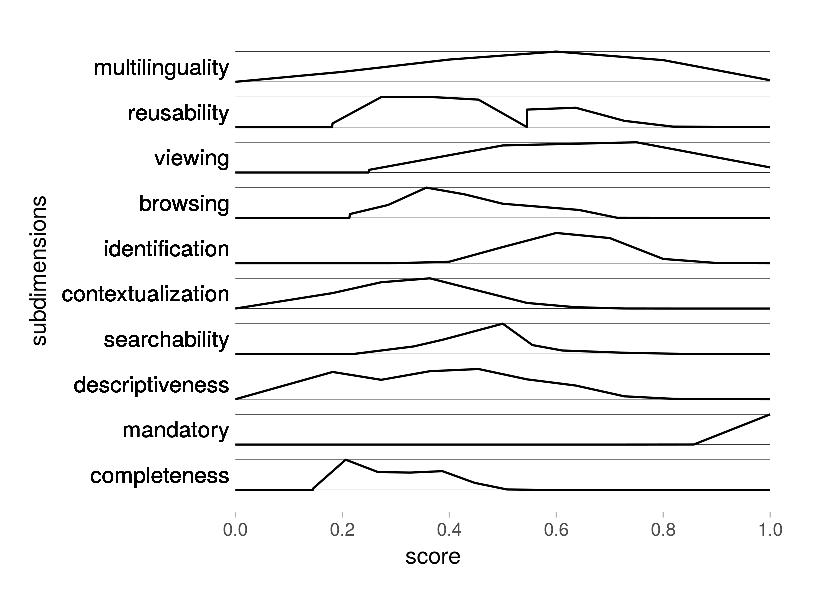
\includegraphics[width=\textwidth]{images/chapter02/subdimensions.eps}
\centering
\caption{The distribution of sub-dimension and 'simple completeness' scores}
\label{figure:subdimensions}
\end{figure}

In the second approach, the main factor is the normalized version of cardinality to prevent the biasing effect of extreme values. Sometimes there are more than one hundred or even a thousand field instances in a single record which would have too much effect on the score, so the tool normalizes them according to table \ref{table:normalization}.

\begin{table}
\caption{Normalization of cardinality}
\label{table:normalization}
\centering
\begin{tabular}{l|c|c|c|c|c}
number of instances & 0 & 1 & 2-4 & 5-10 & 11- \\
\hline
normalized score & 0.0 & 0.25 & 0.50 & 0.75 & 1.0 \\
\end{tabular}
\end{table}

The cardinality-based weight is simple: each field equally counts 1, but the rdf:about field (which identifies the individual entities) counts 10 so that the number of entities is taken into account for the weighting. The equation is

\begin{equation}
c_{cardinality} = \frac{\sum\limits_{i=1}^{d} norm(cardinality_i) \times weight_i}{\sum\limits_{i=1}^{d} weight_i}
\end{equation}

with $d$ as the number of fields, $cardinality_{i}$ as the cardinality of a field, $norm()$ as the normalizing function (see table \ref{table:normalization}) and $weight_i$ as the weight of a field in this computation.

The final equation is the combination of these two approaches where the first approach has a higher weight (so it is more important) than the second one:

\begin{equation}
c_{compound} = \frac{c_{sub-dimensions} + (0.4 \times c_{cardinality})}{1.4}
\end{equation}

\subsection{Implementation}

The data processing workflow has four phases. The current workflow ingests data from a MongoDB database, and stores the extracted records in line-oriented JSON files either in a Linux file system or in a Hadoop File System (using the available resources there is no significant difference in performance between the two, but in other scenarios the Hadoop File System could be a better choice). The record level analyses are written in Java, using the Spark API\footnote{Metadata quality assessment library: https://github.com/pkiraly/ metadata-qa-api, Europeana specific extension: https://github.com/ pkiraly/europeana-qa-api, Apache Spark interface: https://github.com/ pkiraly/europeana-qa-spark. The APIs (and the MARC assessment tool) are available as compiled Java libraries within Maven Central Repository: https://mvnrepository.com/artifact/de.gwdg.metadataqa, so one could use it in 3rd party Java or Scala projects.}. It provides automatic and configurable multithreading, so the tool can make use of the available resources of the environment effectively (either if it is a single machine with a multicore processor or a high performance computing cluster with several nodes). The output of these calculations are CSV files, which are also indexed by Apache Solr for occasional record based retrieval. The tool's quality dashboard makes use of the search and retrieval functionalities in displaying the results, and finding records with given quality metrics. 

The third phase is a statistical analysis of the record level metrics. For datasets and data providers the software is written in R\footnote{source code: https://github.com/pkiraly/europeana-qa-r} and in the Scala implementation of Spark\footnote{https://github.com/pkiraly/europeana-qa-spark/tree/master/scala}. It reads the CSV files generated in the previous phase, and produces CSV and JSON files for storing the results of the calculations and image files for graphs, visualizing central tendencies or other statistical features of the data. R however has a weak point: it works exclusively in memory, so the size of memory limits the size of the dataset it can process. In terms creating statistics for the whole Europeana dataset this is insufficient. For this reason, Scala on Spark is used for all top level aggregations. Scala’s statistical capabilities are not that rich, however, so it does not produce all the metrics that R does.

The last phase is an online statistical dashboard, a light-weighted, PHP and JavaScript based website which displays the output of the previous phases.\footnote{source code: \url{https://github.com/pkiraly/europeana-qa-web}} The technical details of the workflow is documented in \cite{kiraly2015b}. All phases are run in a single commodity hardware (Intel Core i7-4770 Quad-Core processor with 32 GB DDR3 RAM, with Ubuntu 16.04 operating system) which were also used at the same time for other research and development projects, so making the calculations resource-effective was an important software design constraint.

The data source for this calculation is a snapshot of Europeana data. The first snapshot was created at the end of 2015, which contains 46 million records, 1747 datasets and 3550 data providers\footnote{the name of data providers has not been not normalized so far, some organizations have several different names.} (extracted from Europeana's OAI-PMH service). During the project's lifetime additional snapshots have been created, the latest one is from August 2018 (62 million records, 1.27 TB in total, the data source is a replica of Europeana's MongoDB database).\footnote{In order to make the research repeatable, three full data snapshots are available for download at http://hdl.handle.net/21.11101/0000-0001-781F-7 and the first one is archived for long term preservation at the Humanities Data Center, Göttingen: https://hdl.handle.net/21.11101/EAEA0-826A-2D06-1569-0. The format of these snapshot is JSON, one record per line.} DQC aims to introduce a monthly update cycle, so the time span between the updates of the Europeana production database and the refreshing of the data quality dashboard should not be more than one month.

\section{Results}

\subsection{Completeness}

A comparison of the scores of sub-dimension-based (where the field importance counts) and the field-cardinality-based approaches (where the number of field instances counts) reveals that they give different results. While they correlate by the Pearson's correlation coefficient of 0.59, their shape and ranges are different. Because of the nature of the calculation the compound score is quite close to the first approach and the cardinality-based calculation has smaller effect on the final score. The sub-dimension-based scores are in the range of 0.22 and 0.92 while cardinality based scores are in the range of 0.05 and 0.48. The details of the distribution are shown in table \ref{table:completeness_metrics} and figure \ref{figure:completeness}.

\begin{figure}[ht]
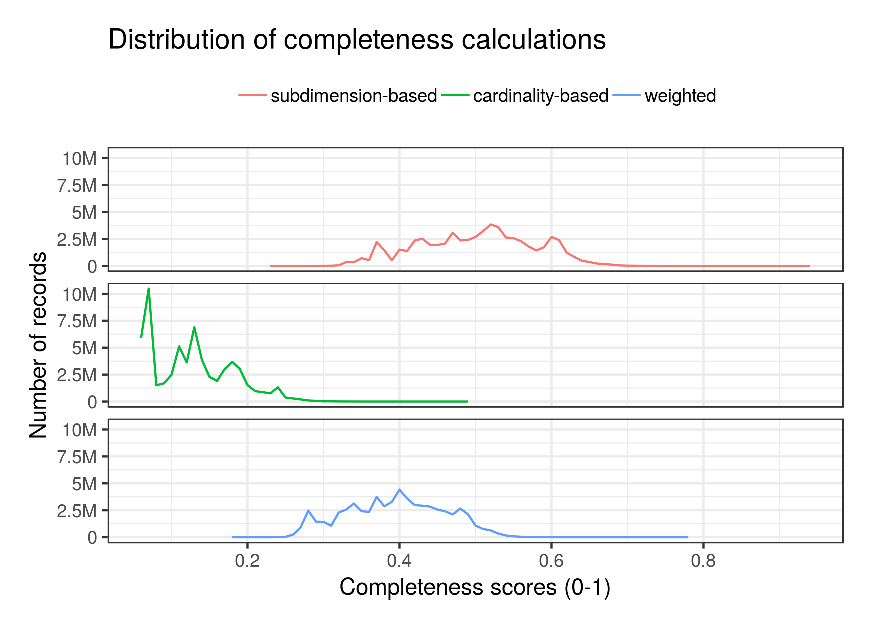
\includegraphics[width=\textwidth]{images/chapter02/completeness-score-histogram.eps}
\centering
\caption{Distribution of completeness calculations}
\label{figure:completeness}
\end{figure}

\begin{table}
\caption{Basic statistics of completeness calculations}
\label{table:completeness_metrics}
\centering
\begin{tabular}{l|c|c|c|c}
metric & mean & std.dev. & min. & max. \\
\hline
sub-dimension-based & 0.50 & 0.07 & 0.22 & 0.93 \\
cardinality-based & 0.12 & 0.05 & 0.05 & 0.48 \\
compound & 0.39 & 0.06 & 0.17 & 0.78 \\
\end{tabular}
\end{table}

There are data providers where all (in some cases more than ten thousand) records have the same scores: they have a uniform structure. Because one simple score is not enough to establish this, the field-level analysis shows that in these collections all the records have the very same (Dublin Core based) field set. On the other end there are collections where both scores diverge a lot. For example, in the identification of sub-dimension a data provider has five distinct values (from 0.4 to 0.8) almost evenly distributed while one of the best collections (of this category) is almost homogeneous: 99.7\% of the records have the same value: 0.9 (even the remaining 0.3\% has 0.8). This means that the corresponding fields\footnote{dc:title, dcterms:alternative, dc:description, dc:type, dc:identifier, dcterms:created, dc:date and dcterms:issued in the Provider Proxy and edm:provider and edm:dataProvider in the Aggregation.} are usually not available in the records of the first dataset, while they are almost always there in the second dataset. The tool provides different graphs and tables to visualize the distribution of the scores. 

From the distribution of the fields the first conclusion is that lots of records miss contextual entities, and only a couple of data providers have 100\% coverage (6\% of the records have \emph{agent}, 28\% have \emph{place}, 32\% have \emph{timespan} and 40\% have \emph{concept} entities). Only the mandatory technical elements appear in every record. There are fields, which are defined in the schema, but not filled in the records and there are overused fields – e.g. dc:description is frequently used instead of more specific fields (such as table of contents, subject related fields or alternative title).

Users can check all the features on the top, collection, and records level on the quality dashboard. Data providers get a clear view of their data, and based on this analysis they can design a data cleaning or data improvement plan.

\subsection{Multilinguality}

DQC has recently published details regarding the results of the multilinguality calculation (see \cite{charles2017} and \cite{kiraly-et-al2018}), so this section presents only a very short summary of the outcome. EDM follows the RDF model for language annotation, so data creators could denote that a string is written in a particular language (e.g. \emph{"Brandenburg Gate"@en}, where 'Brandenburg Gate' is the value of the field, and 'en' denotes English language). This construct is called a tagged literal. DQC found four relevant record-level metrics.

\begin{itemize}
 \setlength{\parskip}{0pt}
 \setlength{\itemsep}{0pt plus 1pt}
\item number of tagged literals
\item number of distinct language tags
\item number of tagged literals per language tags
\item average number of languages per property for which there is at least one language-tagged
\end{itemize}

These metrics were calculated for the Provider Proxy (which is the original data the organizations submit), the Europeana Proxy (which contains enhancements, typically from multilingual vocabularies), and finally for the whole object. The output is summarized in tables \ref{table:multilinguality_metrics} and \ref{table:multilinguality_distribution} and figure \ref{figure:multilinguality}).

\begin{table}
\caption{Metrics of multilinguality (means)}
\label{table:multilinguality_metrics}
\centering
\begin{tabular}{l|c|c|c}
metric & provider & europeana & whole object \\
\hline
number of tagged literals & 5.44 & 64.34 & 69.79 \\
\hline
number of distinct language & 1.67 & 37.92 & 38.79 \\
tags & & & \\
\hline
number of tagged literals & 2.64 & 0.95 & 2.17 \\
per language tags & & & \\
\hline
average number of languages & 1.10 & 28.10 & 20.21 \\
per property for which there & & & \\
is at least one language-tagged & & & \\
 literal & & & \\
\end{tabular}
\end{table}

\begin{figure}[ht]
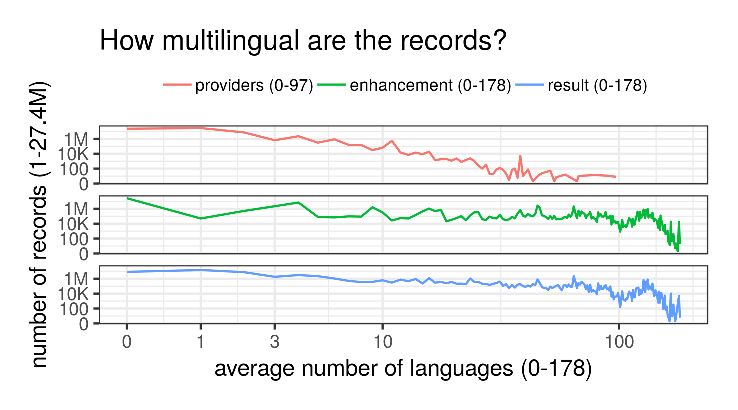
\includegraphics[width=\textwidth]{images/chapter02/multilinguality-summary.eps}
\centering
\caption{Multilinguality}
\label{figure:multilinguality}
\end{figure}

\begin{table}
\caption{Distribution of average number of languages per property}
\label{table:multilinguality_distribution}
\centering
\begin{tabular}{l|r|r|r}
entity & 0 & 1 & 2 or more \\
\hline
Provider Proxy & 22.4M (36.2\%) & 27.3M (44.1\%) & 12.1M (19.6\%) \\
Europeana Proxy & 25.8M (41.7\%) & 49K (0.07\%) & 36.1M (58.2\%) \\
Object & 8.2M (13.3\%) & 14.6M (23.7\%) & 39.1M (63.0\%) \\   
\end{tabular}
\end{table}

Table \ref{table:multilinguality_distribution} reflects that only 20\% of the records have two or more languages per property in the Provider Proxy. After the enhancement process injects external contextual information (about agents, concepts, places and timespans) from multilingual data sources such as DBpedia and other sources into the Europeana records, the overall multilinguality became higher. Not only are the number of fields with two or more language values increased, but the number of records without any language annotation also decreased.

Another finding is that the language tags are not always standardized. Different data providers follow different standards, or use ad-hoc tags. In the whole dataset there are more than 400 different language tags, but several tags denote the same language (e.g. "en", "eng", "Eng" etc. refer to English). A further investigation should analyze records with normalized language tags, to get a more thorough picture of language usage.

\subsection{Uniqueness}

One might recall the example of similar titles mentioned at the beginning of this chapter. To find those records we should calculate the uniqueness of the values. Uniqueness is a positive value in those fields which should describe unique properties of an object, and less positive (or even negative) in those fields which connects records to contextual information where the values should come from a controlled vocabulary, and thus in an ideal case multiple records will share the same terms. In order to effectively establish the uniqueness of a value, one should be able to check a search index with the special requirement that it should index and store field values as a phrase. Since building such an index for the whole dataset would have required more resources than were available for this research, three fields were selected for this task: title, alternative title, and description. In calculating this score a modified version of Solr's relevancy scoring was applied:

\begin{equation}
score(t_f, v_f) = log\left(1 + \frac{t_f - v_f + 0.5}{v_f + 0.5}\right)
\end{equation}

\begin{equation}
uniqueness_f = \left(\frac{score(t_f, v_f)}{score(t_f, 1.0}\right)^3
\end{equation}

$t_f$ is the number of records where field $f$ is available, $v_f$ is the frequency of a value.

As seen in figure \ref{figure:uniqueness-theoretical} the score decreases radically as the field value became more frequent. On the user interface there is a categorization: besides the unique values, there are 5 categories denoted with stars. Table \ref{table:uniqueness-boundaries} displays the category boundaries for these three fields:

\begin{table}
\caption{Uniqueness categories by frequency}
\label{table:uniqueness-boundaries}
\centering
\begin{tabular}{l|c|c|c|c|c}
field & ***** & **** & *** & ** & * \\
\hline
title & 2- & 8- & 37- & 293- & 5226- \\
alternative & 2- & 6- & 23- & 132- & 1514- \\
description & 2- & 7- & 34- & 252- & 4128-
\end{tabular}
\end{table}

\begin{figure}[ht]
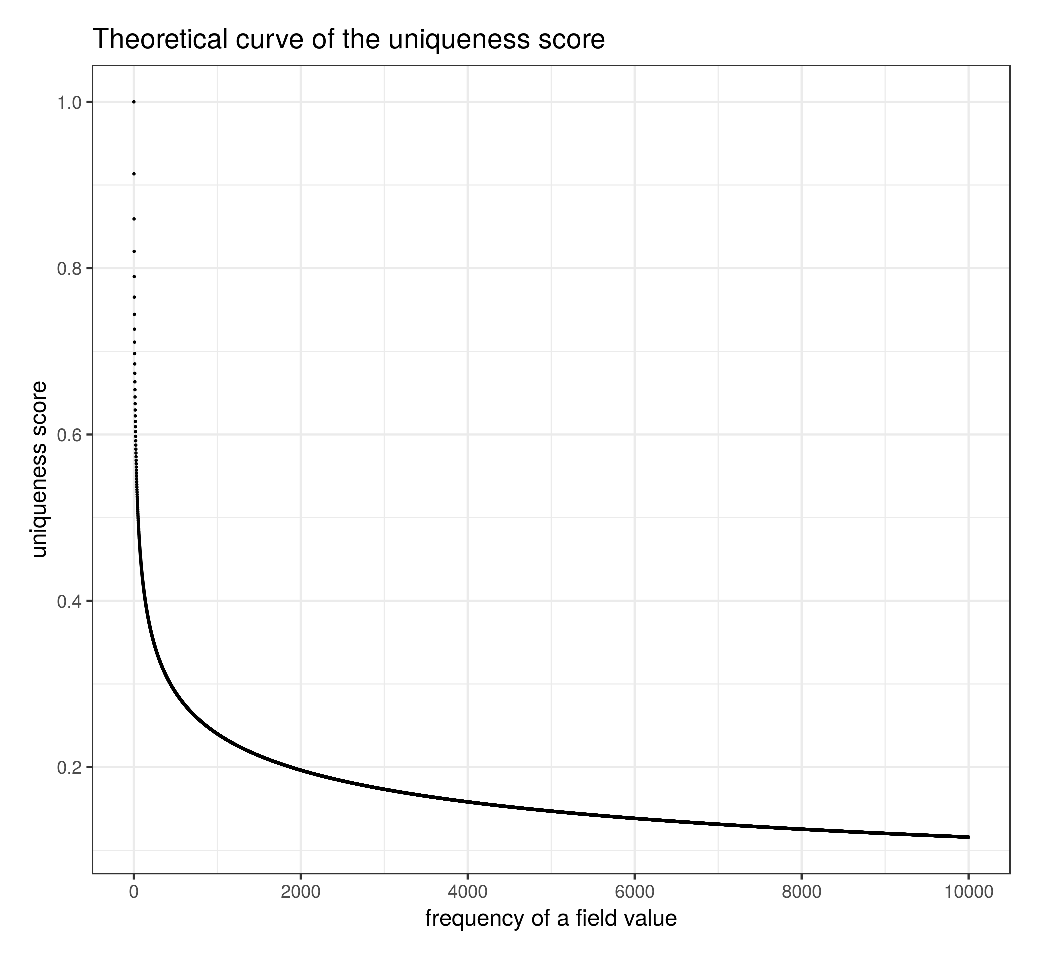
\includegraphics[width=\textwidth]{images/chapter02/uniqueness-theoretical.eps}
\centering
\caption{Theoretical curve of uniqueness score. As frequency of terms gets higher, the uniqueness score get radically smaller towards zero.}
\label{figure:uniqueness-theoretical}
\end{figure}

The result of the categorization is shown in table \ref{table:uniqueness-result}. While the absolute majority of the records in regards to all three fields do contain unique values, there are still millions of records with low scores for one or another field, and moreover there are almost ten thousand records where none of these fields are available. When we examine the three values together (see the last row of the table), and calculate an average of the result, we find that there are 25 million records with unique values in all available fields while on the other side of the scale only 3.62\% of the records are in the lowest category. This means that even if some values are low, most of the time there is at least one field with a less frequent value, so the record has a higher chance to be found by a search term.

\begin{table}
\caption{How unique are Europeana records?}
\label{table:uniqueness-result}
\centering
\begin{tabular}{l|c|c|c|c|c|c}
field & unique & ***** & **** & *** & ** & * \\
\hline
title & 59.4 & 9.5 & 8.3 & 8.7 & 7.1 & 6.6 \\
alternative & 62.4 & 11.2 & 7.1 & 3.6 & 2.7 & 12.7 \\
description & 54.6 & 9.0 & 7.3 & 10.2 & 6.7 & 11.9 \\
together & 45.4 & 10.8 & 15.6 & 18.2 & 6.3 & 3.62
\end{tabular}
\end{table}

From the Solr index one could extract the most frequent terms. Along with the "photograph" example in the introduction there are many frequent phrases in the title field denoting missing information (e.g. ``Unbekannt'', ``Onbekend'' or ``+++EMPTY+++''), collection, journal or institution names (``Journal des débats politiques et littéraires'', ``ROMAN COIN'') or even a general descriptive term (``Porträtt'', ``Château'', ``Plakat'', ``Rijksmonument''). It would require further investigation to filter out those frequent terms which appear in records especially where the other descriptive fields also lack a necessary level of uniqueness. The tool described here provides a solid basis for such an investigation.

\subsection{Record patterns}

What fields make up a typical record? In other words: what fields do data providers actually use? Record patterns are the typical field collocations. Since the completeness measurement counts the existence of all the fields, a map-reduce based analysis could extract these patterns. In this case the mapping function creates the patterns (each pattern is a list of field names available in a particular record) while the reduce-function counts them. In the first iteration it turned out that there were too many similar patterns worthy of grouping together in order to analyze them effectively. A similarity algorithm was therefore applied for clustering the patterns. All patterns were first represented by a string containing zeros and ones. First, all the fields of a collection were collected and sorted by a standard field order. Each field was then categorized into one of three categories: mandatory fields, important fields (those fields which appeared in a sub-dimension) and non-important fields. If the field exists in the pattern it is represented by one or more ones otherwise one or more zeros. The mandatory fields get three characters, the important fields get two, and others gets only one character. This way the patterns having the same important fields and different unimportant fields are closer to each other than patterns sharing the non-important fields. The similarity is calculated by the Jaro-Winkler algorithm. In the visualization (as you can see in figure \ref{figure:patterns}) the clusters are displayed by default, and the user needs to click to display the patterns belonging to a cluster. The table is ordered by the number of records, so the more typical records are on the top. If the field is only available in some records within the cluster, it is grayed (the color is proportional with the number of records). By default the page does not display patterns occuring in less than 1\% of the records.

\begin{figure}[ht]
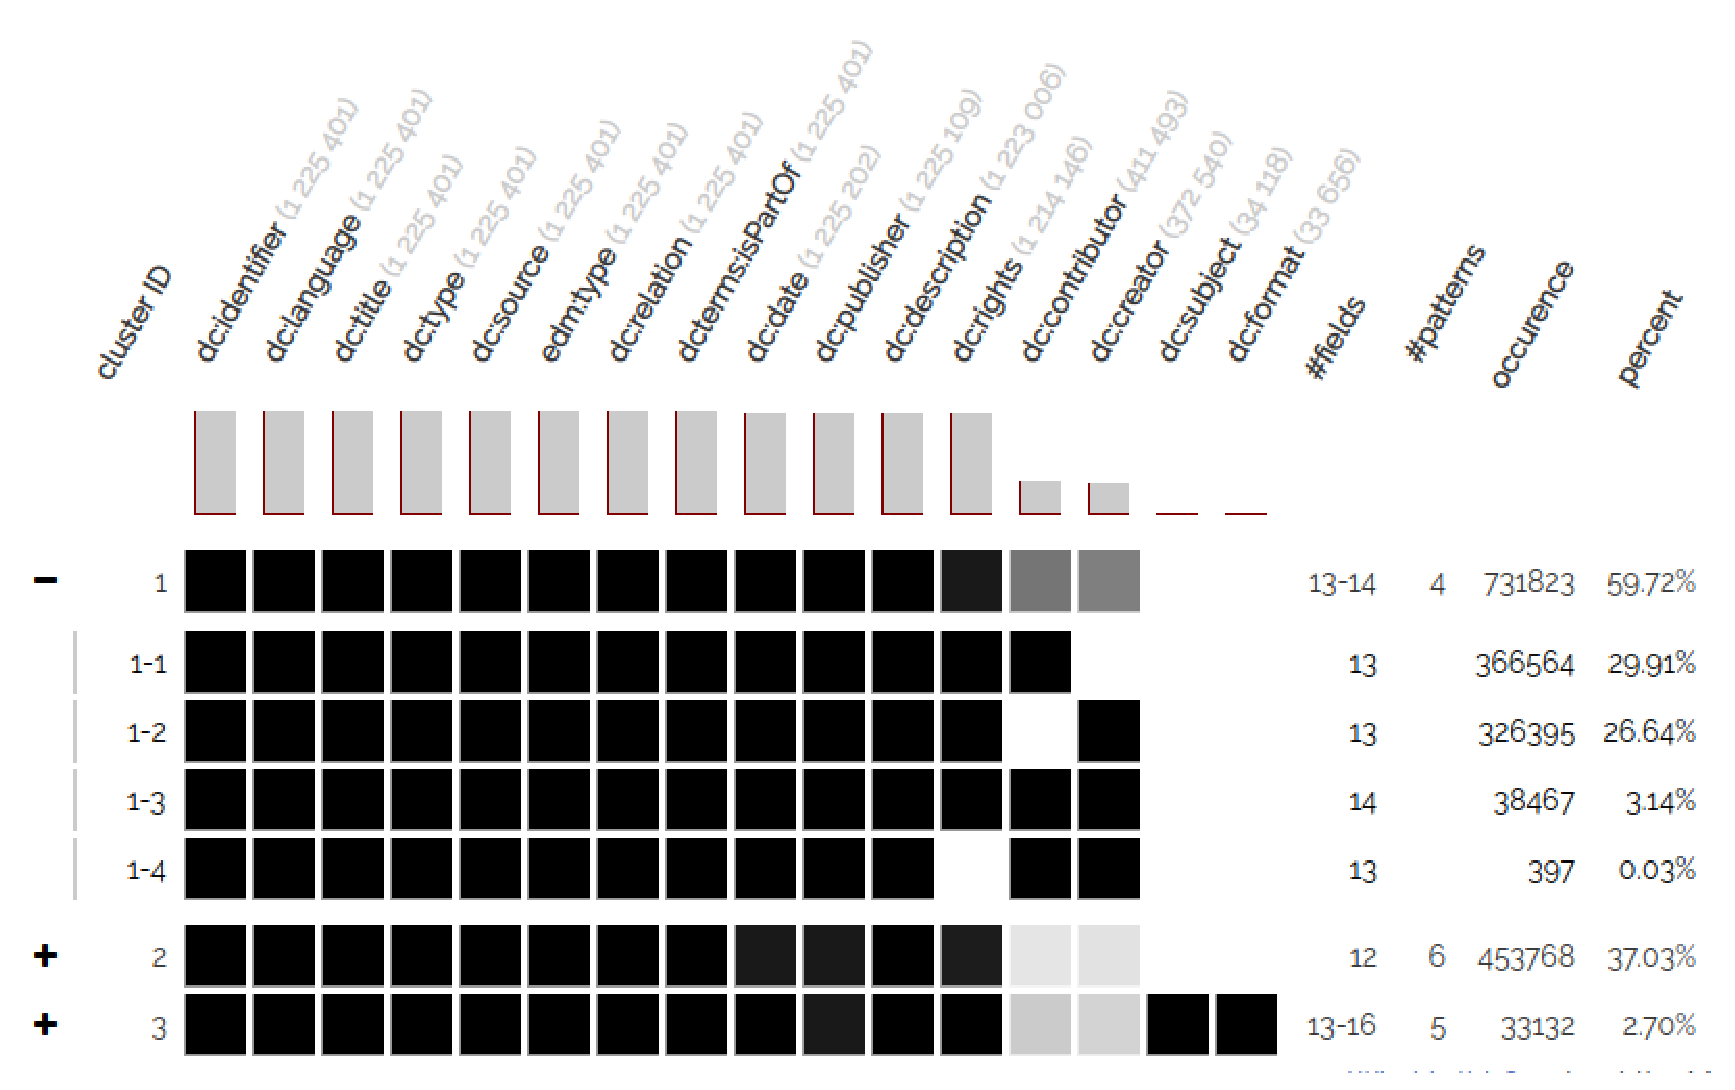
\includegraphics[width=\textwidth]{images/chapter02/clustered-patternsv05.eps}
\centering
\caption{Clustered record patterns. The first line represents a cluster of similar patterns. The next four lines are the patterns belonging to the cluster. The top gray bar represents the frequency of fields in the whole collection.}
\label{figure:patterns}
\end{figure}

Thus far two quality problems were revealed by the use of record patterns. The first problem covers those records which had only a small number of fields. There were more than $150,000$ records having only the following four fields in the Provider Proxy entity: dc:title, dc:type, dc:rights, and edm:type, of which only the first two might contain descriptive information about the object. It is evident that there is a high chance that users would not be able to discover these records by using facets, due to the lack of descriptive information about the object. The second problem is structural homogeneity: each record in some collection always has the same set of fields. There are 906 such data providers in Europeana, but fortunately most of them are relatively small collections, only 26 have more than a thousand records. The biggest homogeneous collection (with over $500,000$ records), however, contains only 5 fields (of which 3 are descriptive). The problem with such a record is that it contains generic fields instead of specific ones (for example it does not make distinctions among conceptual, spatial and temporal subject headings, and puts different contextual information into dc:type or dc:subject).

\section{Further work}

Europeana is currently working on its new ingestion system called Metis\footnote{https://github.com/europeana/metis-framework}, and it will able to integrate the tool described here. It is currently planned that when a new record-set arrives for import the measurement will be launched automatically. The Ingestion Officer can then check the quality report and share both the output and general conclusions with data providers who can then either change their transformation rules or hopefully fix issues with their metadata records if possible.

There are other metrics in addition to the calculation models that were discussed in this chapter, and we are planning to compute them in the near future (e.g. accuracy, information content, timeliness, existence of known metadata anti-patterns). Much of the related literature suggests calculating a top level score, which summarizes all metrics into one final score that characterizes the record’s metadata quality. This could be achieved by weighting the metrics or applying machine learning algorithms, such as Principal Component Analysis \cite{james2013}. It was mentioned previously that the current completeness calculation approach only confirms the existence of a field. The next step on this research front is to extend this model with content evaluation of the relevant fields according to the User Scenarios analysis (\cite{hill-charles-isaac2015}).

In DQC, we also plan to compare the scores with experts’ evaluation and with usage data (log files). Harper ran a test to reveal whether there is a correlation between the usage of an object (the frequency of access via their portal and API) and the scores calculated by a quality assessment conducted by the Digital Public Library of America (which is similar to Europeana regarding to its purpose and its metadata schema). This approach failed partly because there was not enough usage data available at time the research was conducted, however, the proposed method sounds promising, and if Europeana has log files it would be worthwhile to run an experiment.

Other future plans include defining the problem catalogue with W3C’s Shapes Constraint Language \cite{knublauch2017} and publishing the results as linked data fitted to the Data Quality Vocabulary Ontology \cite{albertoni-isaac2016}.

The proposed method could also be used in data collections using other metadata schemas, such as MARC based library catalogues\footnote{Since MARC has lots of strict content related rules, and EDM only has a few, there is a significant distance between the approaches followed in the two projects.}, EAD-based archival collections,\footnote{The biggest European archival collection Archives Portal Europe (http://www.archivesportaleurope.net/) published their data via a REST API under CC0 license.} and others.

\section{Conclusion}

This research sought to rethink the relationship between functionality and metadata schema (together with the DQC) and a framework was implemented that proved successful in measuring structural features that correlate with metadata issues. The user of the framework is able to select between low and high quality records. According to our original hypothesis, structural features such as field existence and cardinality correlated with metadata quality, and this ultimately proved to be true. In addition, this work also extended the volume of records analyzed by introducing big data tools that were not mentioned previously in the literature.

Although this research focused on a particular dataset and metadata schema, the applied method is based on generalized algorithms so it could also be applied to other data schemas. Several Digital Humanities studies (some examples: KOLIMO (Corpus of Literary Modernism)\footnote{https://kolimo.uni-goettingen.de/}, \cite{strezoski2017}, \cite{schmidt2017}) based on schema defined cultural databases. The research process could also be improved by finding the weak points of the sources, making the conclusions more reliable, and -- reflecting on Felix Rau's tweet quoted at the beginning of this chapter -- by forming more realistic assumptions about the data.

\section*{Acknowledgment}
The first author would like to thank to all the past and current members of the Europeana Data Quality Committee, to the supervisors of his PhD research, Gerhard Lauer, and Ramin Yahyapour, to Jakob Voß, Juliane Stiller, Mark Phillips for providing feedback, to Christina Harlow and Zaveri Amrapali for general inspiration, and to Felix Rau for the motto and to GWDG for supporting the research.

% \bibliographystyle{acm}
% \bibliography{bibliography-for-papers}
